\documentclass[letterpaper]{article}

\usepackage{aaai}
\usepackage{times}
\usepackage{helvet}
\usepackage{courier}
\usepackage{graphicx}
\usepackage{stfloats}
\usepackage{color}

% \usepackage{float}
% \floatstyle{boxed} 
% \restylefloat{figure}

\usepackage[noend,linesnumbered,algoruled]{algorithm2e}
% %%%%%%%%%%%%%%%%%%%%%%%%%%%%%%%%%%%%%%%%%%%%%%%%%%%%%%
% PDFMARK for TeX and GhostScript
% Uncomment and complete the following for metadata if
% your paper is typeset using TeX and GhostScript (e.g
% if you use .ps or .eps files in your paper):
% \special{! /pdfmark where
% {pop} {userdict /pdfmark /cleartomark load put} ifelse
% [ /Author (John Doe, Jane Doe)
% /Title (Paper Title)
% /Keywords (AAAI, artificial intelligence)
% /DOCINFO pdfmark}
% %%%%%%%%%%%%%%%%%%%%%%%%%%%%%%%%%%%%%%%%%%%%%%%%%%%%%%
% PDFINFO for PDFTeX
% Uncomment and complete the following for metadata if
% your paper is typeset using PDFTeX
% \pdfinfo{
% /Title (Input Your Title Here)
% /Subject (Input The Proceedings Title Here)
% /Author (First Name, Last Name;
% First Name, Last Name;
% First Name, Last Name;)
% }
% %%%%%%%%%%%%%%%%%%%%%%%%%%%%%%%%%%%%%%%%%%%%%%%%%%%%%%
% Uncomment only if you need to use section numbers
% and change the 0 to a 1 or 2
% \setcounter{secnumdepth}{0}
% %%%%%%%%%%%%%%%%%%%%%%%%%%%%%%%%%%%%%%%%%%%%%%%%%%%%%%


\newcommand{\from}[2]{\textcolor{red}{\noindent\textbf{//}\textbf{Note
      from #1:}\textsc{ #2}\textbf{//}}}
      
      \newcommand{\fw}[1]{\texttt{#1}}




\begin{document}

\title{Towards a Cognitive System That Can Recognize Spatial Regions Based on Context}
% \title{Representing and Reasoning About Spatial Regions Defined by Context}
% \title{Context-Dependent Spatial Regions}

\author{}


\maketitle
\begin{abstract}
In order to collaborate with people in the real world, cognitive systems must be able to represent and reason about spatial regions in human environments. Consider the command \emph{``go to the front of the classroom''}. The spatial region mentioned (the front of the classroom) is not perceivable using geometry alone. Instead it is defined by its functional use, implied by nearby objects and their configuration. In this paper, we define such areas as \textit{context-dependent spatial regions} and present a cognitive system able to learn them by combining qualitative spatial representations, semantic labels, and analogy. The system is capable of generating a collection of qualitative spatial representations describing the configuration of the entities it perceives in the world. It can then be taught context-dependent spatial regions using \textit{anchor points} defined on these representations.  From this we then demonstrate how an existing computational model of analogy can be used to detect context-dependent spatial regions in previously unseen rooms. To evaluate this process we compare detected regions to annotations made on maps of real rooms by human volunteers.
\end{abstract}

\section{Introduction}

Consider a janitorial robot cleaning a classroom. While performing this task, it encounters a teacher working with a student. The teacher tells the robot to ``start at the front of the classroom'', expecting it to go to the front of the classroom and begin cleaning that area. This response requires that the robot is able to \emph{determine the spatial region in the environment that satisfies this concept}.

The ability to understand and reason about \textit{spatial regions} is essential for cognitive systems performing tasks for humans in everyday environments. Some regions, such as whole rooms and corridors, are defined by clearly perceivable boundaries (e.g. walls and doors). However, many regions to which humans routinely refer are not so easily defined. Consider, for example, the aforementioned region \textit{the front of the classroom}. This region is not perceivable using just the geometry of the environment. Instead, it is defined by the objects present in the room (chairs, a desk, a whiteboard), their role in this context (seats for students to watch a teacher who writes on the whiteboard) and their configuration in space (the seats point toward the whiteboard). We refer to such regions as \textit{context-dependent spatial regions} (CDSRs). 

Current cognitive systems are not capable of representing and reasoning about CDSRs, yet it is an important ability. If cognitive systems are to collaborate with humans in everyday environments then they must be able to understand and refer to the same spatial regions humans do. Many regions are best defined in a context-dependent manner, for example, a kitchen in a studio apartment, an aisle in a church or store, behind enemy lines in a military engagement, etc. In order to represent and reason about such regions, cognitive systems must integrate different types of information, including geometric, semantic, and functional knowledge. Creating systems able to integrate such a range of information is a key challenge in the cognitive systems paradigm \cite{langley:inpress}.

This paper presents an artificial cognitive system (specifically a mobile robot) able to represent and reason about CDSRs. Our approach is founded on two assumptions. The first assumption is that CDSRs can be defined using \emph{qualitative spatial representations} (QSRs) corresponding to sensor data of the system~\cite{Cohn:2001}. The second assumption is that semantically and geometrically similar areas (e.g. two different classrooms) will feature similar CDSRs, and that these similarities can be recognised through \emph{analogy}. The rest of the paper is structured following these assumptions. Section~\ref{sec:qsr-gen} describes how we generate QSRs from sensor data taken from an existing, state-of-the-art, cognitive system and use these to define CDSRs. Section~\ref{sec:analogy} then describes how we use the structure-mapping model of analogy \cite{Gentner1983a} to transfer a CDSR from a labelled example to a new situation. Section~\ref{sec:example} presents a worked example of the entire process, and Section~\ref{sec:evaluation} evaluates our system in comparison to data from human subjects performing the same task.


\section{Metric to Qualitative Representations}\label{sec:qsr-gen}

% Our approach to representing and reasoning about context-dependent spatial regions requires the existence of qualitative spatial representations~\cite{Cohn:2001} describing the relationships between the entities a cognitive system perceives (including objects, groups, and regions). By adding semantic labels, or types, to each entity, we are able to reason about the geometric \emph{and} conceptual characteristics of the system's environment. The following sections describe how we generate appropriate qualitative spatial representations using the spatial model of an existing, state-of-the-art, cognitive system.

The context which defines a CDSR is a combination of the functional and geometric properties of a room, i.e. what can be done there and where. In this work we implicitly represent context using the types of objects present in a room and their location relative to each other. The following sections describe how we construct symbolic representations of these ingredients of context from robot sensor data. 

\subsection{The Dora System}

We base our work on Dora, a mobile cognitive robot with a pre-existing multi-layered spatial model~\cite{Hawes/etal:2011}. In this paper, we draw on the metric map from this model. For more information on Dora's other competences, see recent papers, e.g.~\cite{Hawes/etal:2011,Hanheide/etal:2011}.

Dora's metric map is a collection of lines in a 2D global coordinate frame. Two example maps are pictured in Figure~\ref{fig:rooms}. These lines are generated by a process which uses input from the robot's odometry and laser scanner to perform simultaneous localization and mapping (SLAM). Lines in this SLAM map represent features extracted from laser scans wherever a straight line is present for long enough to be considered permanent. In practice, lines are generated at the positions of walls and any other objects that are flat at the height of the laser (e.g. bins, closed doors etc.). The robot's location in the metric layer is represented as a 2D position plus an orientation. 

Dora is capable of using vision to recognize pre-trained 3D object models. Recognition can either be triggered through autonomous visual search or at a user's command. When an object is detected it is represented in the metric map 
by placing a copy of the model at the detected pose. The recognizer associates each object with a semantic type that was provided during a training phase.

To enable us to generate a range of different evaluation situations in a reasonable length of time, we have generated data from Dora in both real rooms and in simulation. Simulation is performed using the Player/Stage hardware abstraction layer~\cite{GerkeyVaughanHoward03} allowing us to run the system \emph{mostly unchanged} in a pre-defined environment. Also, to enable us to detect a wider range of objects than is usually possible (from armchairs to whiteboards), we used a simulated object recogniser in all runs. The recogniser was configured with types and positions of objects in the environment and was guaranteed to detected them when the robot was orientated towards them. This eliminated any errors from the recognition process, but was still influenced by errors in robot localisation.

\subsection{Qualitative Spatial Representation Extraction}

Given data from Dora's spatial model we compute a set of spatial relations between each pair of adjacent objects. For each object in the room we compute 8 spatial relations between that object and each of the objects adjacent to it; adjacency is determined by creating a voronoi diagram as is standard geometric reasoning \cite{Forbus/etal2003}. The relations we compute between a given object and one of the objects adjacent to it are analogous to the cardinal and intermediate points on the compass when the compass is centered on the object. The canonical directions of these relations are defined using the following vectors: $<0,1>$, $<1,1>$, $<1,0>$, $<1,-1>$, $<0,-1>$, $<-1,-1>$, $<-1,0>$, $<-1,1>$.

To compute these relations we first, extract the object and room entities from the sensor data. Next, for the room, we compute its region as a convex hull. Taking each object in the room in turn to be the current landmark, we translate the origin of the room to the landmark's centroid. This translation results in the coordinates of the all the other objects in the room being translated into a frame of references whose origin is the centroid of the landmark.  For each object adjacent to the landmark we compute the 8 relations by computing the inner angle between the vector from the origin (the landmark's centroid) and the object's location and the direction vector of the relation, as defined above. This angle is computed by taking the dot product of these two vectors. $\dots$



%%\from{Nick}{I have changed the below paragraph to match the actual numbers and images. I've marked what I changed}
%%Desk 1 and Desk 2 are not labeled in the Figure.

%Consider the situation in Figure~\ref{fig:dora-spatial} where the robot is facing two desks in a row\footnote{Please note that although the desks in front of the robot in Figure~\ref{fig:dora-spatial} appear distributed left to right from the robot's current position, they are actually distributed bottom to top, according to our definitions, in the global coordinate frame.}. Because we represent the desks as distinct points, \fw{(rcc8-DC Desk1 Desk2)} states that they are disjoint. To account for their relative positions, neither \fw{(leftOf Desk1 Desk2)} nor \fw{(leftOf Desk2 Desk1)} are true because the x coordinate of \fw{Desk1} is within a threshold of the x coordinate of \fw{Desk2}. The statement \fw{(below Desk1 Desk2)} is true because \fw{Desk1} has a lower y coordinate. Each desk is also related to the room by the non-tangential proper part relation, \fw{rcc8-NTPP}. These qualitative spatial relationships provide the structure necessary for analogical processing.


\subsection{Representing CDSRs}

We use \textit{anchor points}~\cite{Klenk/etal2005} to define the boundaries of CDSRs. Anchor points are symbolic descriptions which link a conceptual entity to a perceived entity. The perceived entities we use are the objects recognised by Dora, and the room itself. The room representation is created by putting a convex hull around the lines in Dora's SLAM map. Anchor points are created from perceived entities using unary functions, e.g. \fw{(XMaxYMostFn Desk1)} represents the point on the \fw{Desk1} with the largest x coordinate taken from the set of points with a y coordinate within 5\% of the maximum y coordinate. Anchor points are linked to particular CDSRs using a \fw{boundarySegment} ternary relation. After we have defined the boundary of the region, we assign it a semantic label using the \fw{regionType} relation. Therefore, each CDSR has one type and a variable number of boundary segments.

\begin{figure}[h]
	{\fontsize{8}{8} %%Because aaai.sty overrides usual font size commands

\fw{(regionType CDSR9 FrontRegion) \\
(boundarySegment CDSR9 \\
\hspace*{2em}(YMaxXFewestFn Room3) \\
\hspace*{2em}(YMinXFewestFn Room3)) \\
(boundarySegment CDSR9 \\
\hspace*{2em}(YMinXFewestFn Room3) \\
\hspace*{2em}(YMinXFewestFn Group1))
}
}
  \caption{Three of the five expressions representing the front of the classroom context-dependent region \fw{CDSR9}}
  \label{fig:cdsr-reps}
\end{figure}

Figure \ref{fig:cdsr-reps} contains three of the five expressions defining the front of classroom \fw{Room3} which is pictured in the top of Figure~\ref{fig:rooms}. The boundary segments (shown in orange in Figure~\ref{fig:rooms}) define the extent of the region. \fw{(YMaxXFewestFn Room3)} and \fw{(YMinXFewestFn Room3)} are the points with the highest and lowest y coordinate out of the set of points within 5\% of the minimum x coordinate of \fw{Room3}. The next segment connect the lower left coordinate in the figure to the \fw{(YMinXFewestFn Group1)}, where \fw{Group1} includes the eight desks. There are two more boundary segments completing a polygon for this region. The semantic label \fw{FrontRegion} ties this polygon to a conceptual region, "the front of the room". This definition for the front of the room is specific to \fw{Room3} and its entities. It is clearly context-dependent because its extent is dependent on the arrangement of the anchor points used to define its boundary. If the desks were in a different position then the region would cover a different extent (e.g. if they were further to the left then the region would be smaller). 



\section{Analogical Transfer of Spatial Regions}\label{sec:analogy}


We assume that a cognitive system will have a way of initially acquiring examples of CDSRs, e.g., by being taught through dialogue, sketching, or hand-coding. To avoid burdening potential users with the task of teaching the system every CDSR individually, it is desirable for a cognitive system to be able to automatically recognize similar regions after initial training. For example, after a janitorial robot has been taught where the front of one classroom is, it should be able to identify the fronts of other classrooms in the building. We have chosen \emph{analogy} as the approach our system will use to solve this problem, as analogy has been previously used to successfully combine semantic and geometric information in spatial reasoning tasks~\cite{Lockwood/etal2008}.


Analogy is an essential cognitive process. In humans, analogical processing has been observed in language comprehension, problem-solving, and generalization \cite{Gentner2003}. The structure-mapping theory of analogy and similarity postulates this process as an alignment between two structured representations, a \textit{base} and a \textit{target} \cite{Gentner1983a}. 
% This alignment process is governed by three constraints: \textit{identicality}, \textit{parallel connectivity}, and \textit{one-to-one mapping}. The identicality constraint provides a strong preference for only allowing identical predicates to match. Parallel connectivity states that if two predicates are matched then their arguments must also match. The one-to-one mapping constraint requires that each element in the base corresponds to at most one element in the target and vice versa. To select between competing mappings, the \textit{systematicity} principle prefers mappings that are highly interconnected and contain deep chains of higher order relations over mappings with an equal number of relations which are independent from each other.
We use the Structure-Mapping Engine (SME) \cite{Falkenhainer1989a} to perform analogical matching in our system. Given base and target representations as input, SME produces one or more mappings. Each mapping is represented by a set of \textit{correspondences} between entities and expressions in the base and target structures. Mappings are defined by expressions with an identical relation and corresponding arguments. When provided with expression strengths, such as, our spatial relationships, SME prefers mappings with closely aligned fact strengths. SME can be given \textit{pragmatic constraints} that require certain entities in the base to be included in the mapping. Mappings also include \textit{candidate inferences} which are conjectures about the target using expressions from the base which, while unmapped in their entirety, have subcomponents that participate in the mapping's correspondences. SME operates in polynomial time, using a greedy algorithm \cite{Forbus/etal1994}.

\begin{figure}[h]
  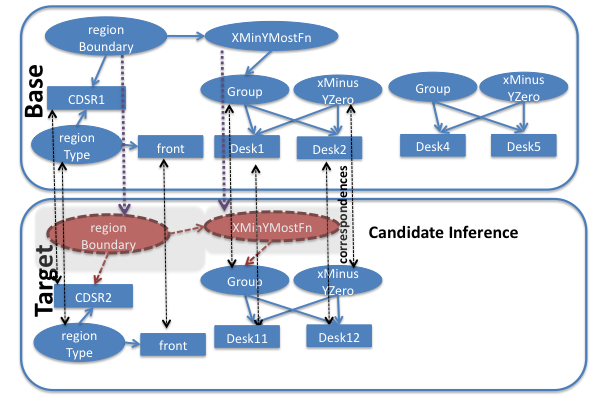
\includegraphics[width=\columnwidth]{images/AnalogyDiagram.png}
  \caption{Analogical mapping between six base expressions and three target expressions. }
  %Ovals and squares represent relations and entities respectively. Black dashed bi-directional arrows are the correspondences between the base and target, and the red dashed objects represent a candidate inference projected into the target.
  
  \label{fig:analogy}
\end{figure}


Figure \ref{fig:analogy} illustrates a sample mapping between six base expressions and three target ones. Each oval represents a predicate, and the entity arguments are represented by squares. SME generates a mapping between the base expressions \fw{(group Desk1 Desk2)} and  \fw{(xMinusYZero Desk1 Desk2)}, and the  target expressions \fw{(group Desk11 Desk12)} and \fw{(xMinusYZero Desk11 Desk12)} as well as between the \fw{regionType} expressions in each case in the following manner. First, the predicates of these expressions are placed in correspondence, as identical predicates are preferred by SME. Then SME aligns the arguments of the aligned predicates, \fw{Desk1} with \fw{Desk11},  \fw{Desk2} with \fw{Desk12}, and \fw{CDSR1} with \fw{CDSR2}. While there is another \fw{XMinusYZero} statement in the base about two desks, it cannot correspond to either of the target expressions in the same mapping due to the one-to-one constraint in SME which allows each element in the target to map to at most one element in the base and vice versa. In Figure \ref{fig:analogy}, the correspondences are highlighted by the hashed bi-directional arrows. Next, SME creates a candidate inference for the boundary segment expression, because both the mapped \fw{Group} and \fw{regionType} predicates participate in the mapping. The candidate inference is shown in red in the figure. Note that inference is selective, with no candidate inferences generated for the entirely unmapped expressions. %Next, we describe how we use the results of an analogy to infer a context-dependent spatial region in the target.
 
% It feels odd having this as a separate subsection
%\subsection{Initial Approach}\label{sec:approach}

In our system, the base and target representations consist of the entities Dora has perceived in two different rooms, the QSRs between them and any groups that have been identified. The base also contains a labeled CDSR of the type sought in target. The result of running SME on these representations is a set of correspondences between the base and target, and a set of candidate inferences about the target. We use these to transfer the CDSR from base to target (i.e. recognizing the CDSR in the target) as follows. First, we identify the CDSR of the sought type in the base and use SME's pragmatic constraints to ensure that the entities referred to its anchor points participate in the mapping. To transfer the CDSR to the target, we collect the candidate inferences that result from \fw{boundarySegment} statements mentioning the base CDSR. The second and third arguments of these candidate inferences are anchor points in the target environment. We use these to define the boundary of the CDSR in the target.

\section{Example System Run}\label{sec:example}



\begin{figure}
	% can swap these 2 lines for different presentations - and colours!
 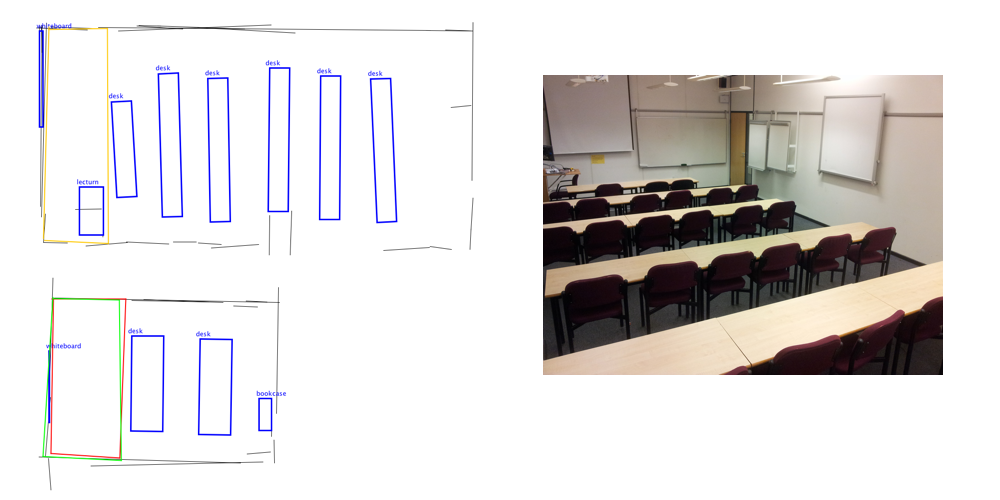
\includegraphics[width=\columnwidth]{images/worked-example.png}
  % 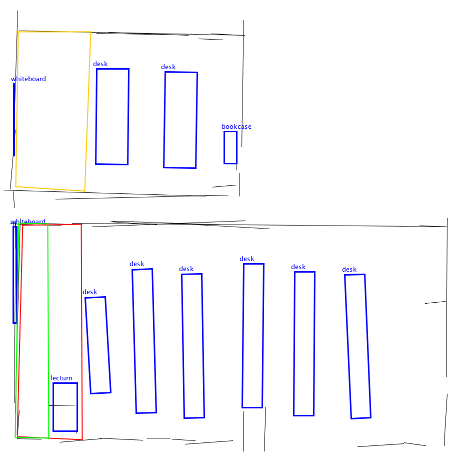
\includegraphics[width=\columnwidth]{images/worked-example-rooms.png}
  \caption{Maps of 2 real classrooms generated by our system. The lines around the perimeter are walls, the unfilled polygons are the outlines of objects and the filled polygons are CDSRs. The maps show an expert-annotated CDSR (red, top image), a subject-annotated CDSR (blue, bottom image) and a CDSR transferred by analogy (green bottom image). The classroom used to generate the bottom classroom is pictured in Figure~\ref{fig:ug40}.}
  \label{fig:rooms}
\end{figure}

\begin{figure}
  
\includegraphics[width=\columnwidth]{images/ug40.png}
  \caption{One of the classrooms used in our evaluation. This image was presented to subjects who were asked to annotate a copy of the image in the bottom half of Figure~\ref{fig:rooms}. The inset shows a screenshot from the data collection webpage.}
  \label{fig:ug40}
\end{figure}



To elucidate the workings of our system, we now present an example of how it can transfer a CDSR describing the front of a known classroom (the base) to a new classroom (the target). 

We first create the base and target representations by running Dora in the two different classrooms. These are pictured in the top and bottom of Figure~\ref{fig:rooms} respectively. In each case, Dora is manually driven around the room to allow it to create a metric map. Once the map is created, Dora is then positioned such that the objects are observable and the visual recognition system is run. The map and object data that result from this are then passed on to the QSR generator. In the base case, Dora perceives 8 individual desks, a group entity containing these desks and the room area. To this we add the CDSR representing the front of the room. The case includes a total of 50 expression relating the 20 entities. Six of these expressions are used to define the boundary segments and CDSR representing the front of the room. The target case includes 26 expressions and 11 entities.

SME generates an analogy between the base and target cases enabling the transfer of the symbolic description of the front of the room to the new situation requiring \fw{Room3} and \fw{Group1} participate in the mapping as they are referenced by the anchor points in the base. The resulting analogy includes 26 correspondences between the entities and expressions and 32 candidate inferences. Four of these candidate inferences define the CDSR in the target with anchor points to the group of desks and the room in the target. The green region in the lower image of Figure \ref{fig:rooms} illustrates the transferred CDSR.

% coming soon

We have implemented our switching continual approach in the MAPSIM
environment~\cite{brenner:nebel:jaamas09},
using \system{dlib-ml}~\cite{king:2009} for belief
revision. Sequential sessions use a modified version of Fast
Downward~\cite{fast-downward}, and DT sessions use our own contingent
procedure. We also implemented a simple dual-mode replanning {\em
baseline} approach. Here, when a switching action is scheduled for
execution the DT session executes a single entropy reduction action,
that directly senses an active assumption -- i.e,. We say a fact can
be directly sensed, if there is a DTPDDL {\em sense} declaration that
mentions the fact in its precondition.  Control is then immediately
returned to a new sequential session.


We evaluate our approaches in robot exploration tasks from home and
office environments. Spatially, these consist of {\em rooms}
(office/kitchen/etc), and an underlying topological map that models
smaller areas of space, called {\em places}, and connectivity between
those. The mobile {\em robot} and {\em visual objects} inhabit the
topological space, the latter indicate the category of space they
inhabit -- e.g., spoons are likely to be in kitchens. By examining
view cones at places for particular objects, the robot is able to: (1)
categorise space at high (room) and low (place) levels, and (2) find
objects for the user, exploiting information about object
co-occurrence and room categories for efficiency. Also, in the
presence of a person, the robot can ask them about the category of the
current room.


We compare switching with the {\em baseline} in several realistic
tasks, with the number of rooms ranging from 3 (12-places, 16-objects,
$|$states$|$ $>10^{21}$) to 6 (26-places, 21-objects, $|$states$|$
$>10^{36}$). We also compare those systems with an approximately
optimal policy computed using Smith's {\sc zmdp} for small 2 room
problems (4-places, 3-objects, $|$states$|$ $\simeq 5000$). For or
experiments we model three sensors: {\em Reliable} sensors have a
$0.1$ probability of a false negative, {\em semi-reliable} have a
chance of $0.3$ of false negative and $0.1$ of false positive , and
finally {\em noisy} sensors with probabilities of $0.5$ and $0.2$
respectively. Each object class is assigned one sensor model, so
e.g. cornflakes may be harder to detect than refrigeratos. To
determine the influence of the sensor model, we performed several
experiments where we only changed the difficulty of the target
object(s). All non-target objects remain unchanged so the planner may
exploit object co-occurances with reliable objects to compensate for
the increased sensor noise.


We evaluate with DT sessions taking $b_0$ admitting between 20 and 100
abstract states with non-zero probability. We run 50 simulations in
each configuration, and have a timeout on each simulation of 30
minutes (1800 seconds)\footnote{All experiments were conducted on a
 2.66GHz Intel Xeon X5355 using one CPU core.}. The continual planning
times are reported in Figure~\ref{fig:results-time}, and the quality
data in Figure~\ref{fig:results-quality}.
%%
For each task, the goal is to find one or several objects and report
their position to a user. Usually there is a non-zero probability that
no plan exists, as the desired object might not be present in the
environment.
% MOG: I didn't do  evaluations for those, so let's remove them
% Item~$f$ reports for tasks requiring indirect sensing,
% where the robot must relocate to a room with a particular category
% (e.g. kitchen). the {\em baseline} is not able to complete Item~$f$,
% so is omitted from that reporting.  
Because reward is only allocated
once, on the achievement of the goal,  we find it
intuitive to report average plan costs and the success rates in
problems that admit a solution (i.e., positive reward scaled by a
constant factor).

\begin{figure}[h!]
  % \centering
  % 
\includegraphics{dora1-time}\hfill
  % \vspace{2mm}
  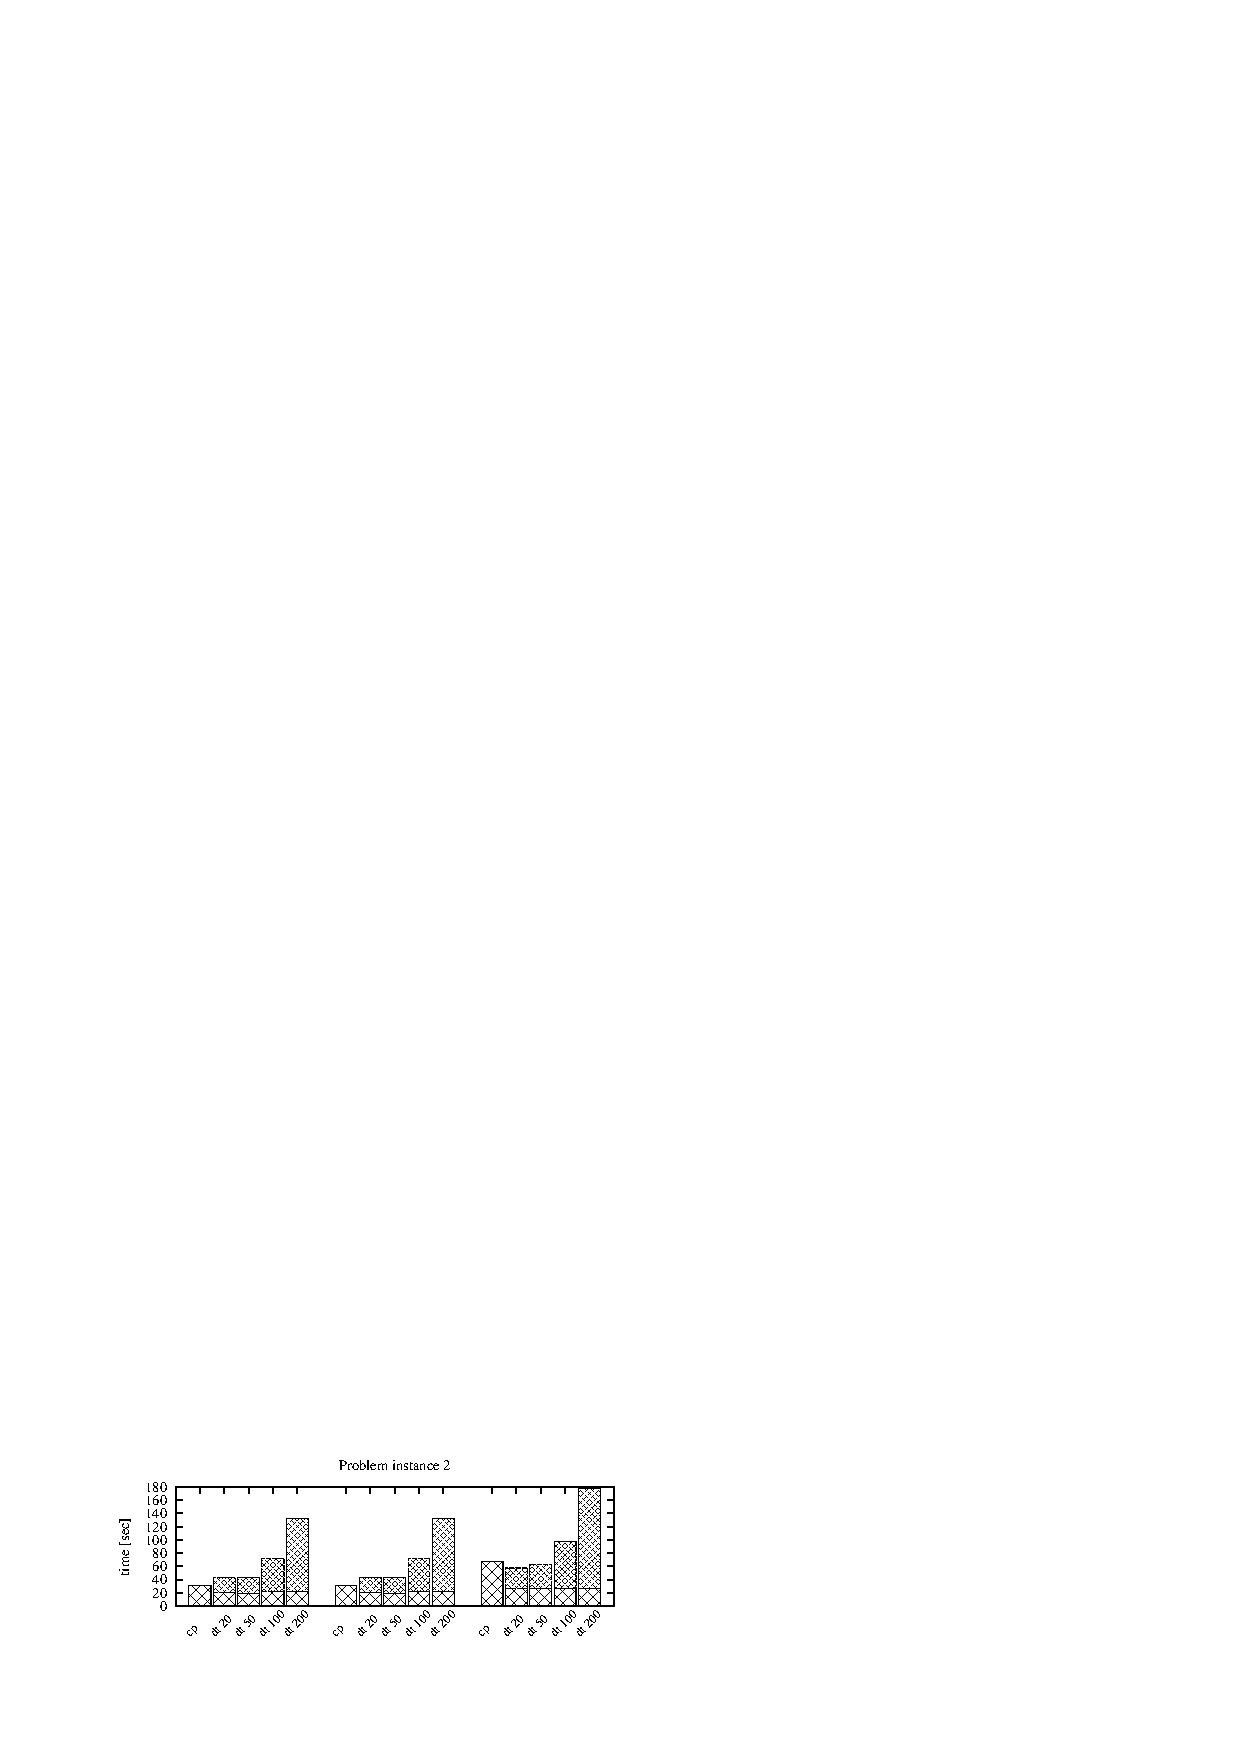
\includegraphics{dora2-time}\hfill
  % \vspace{2mm}
  
\includegraphics{dora3-time}\hfill
  % \vspace{2mm}
  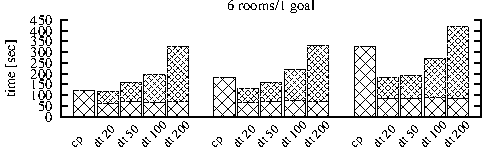
\includegraphics{dora4-time}\hfill
  \vspace{2mm}
  
\includegraphics{dora56-time}\hfill
  % \vspace{2mm}
  % 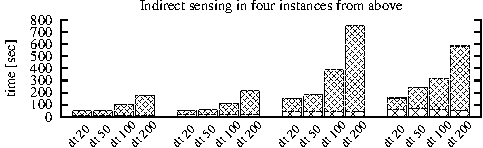
\includegraphics{dora-cat-time}\hfill
  \caption{Average runtime}
  \label{fig:results-time}
\end{figure}

\begin{figure}[h!]
  % \centering
  % 
\includegraphics{dora1-quality}\hfill
  % \vspace{2mm}
  % 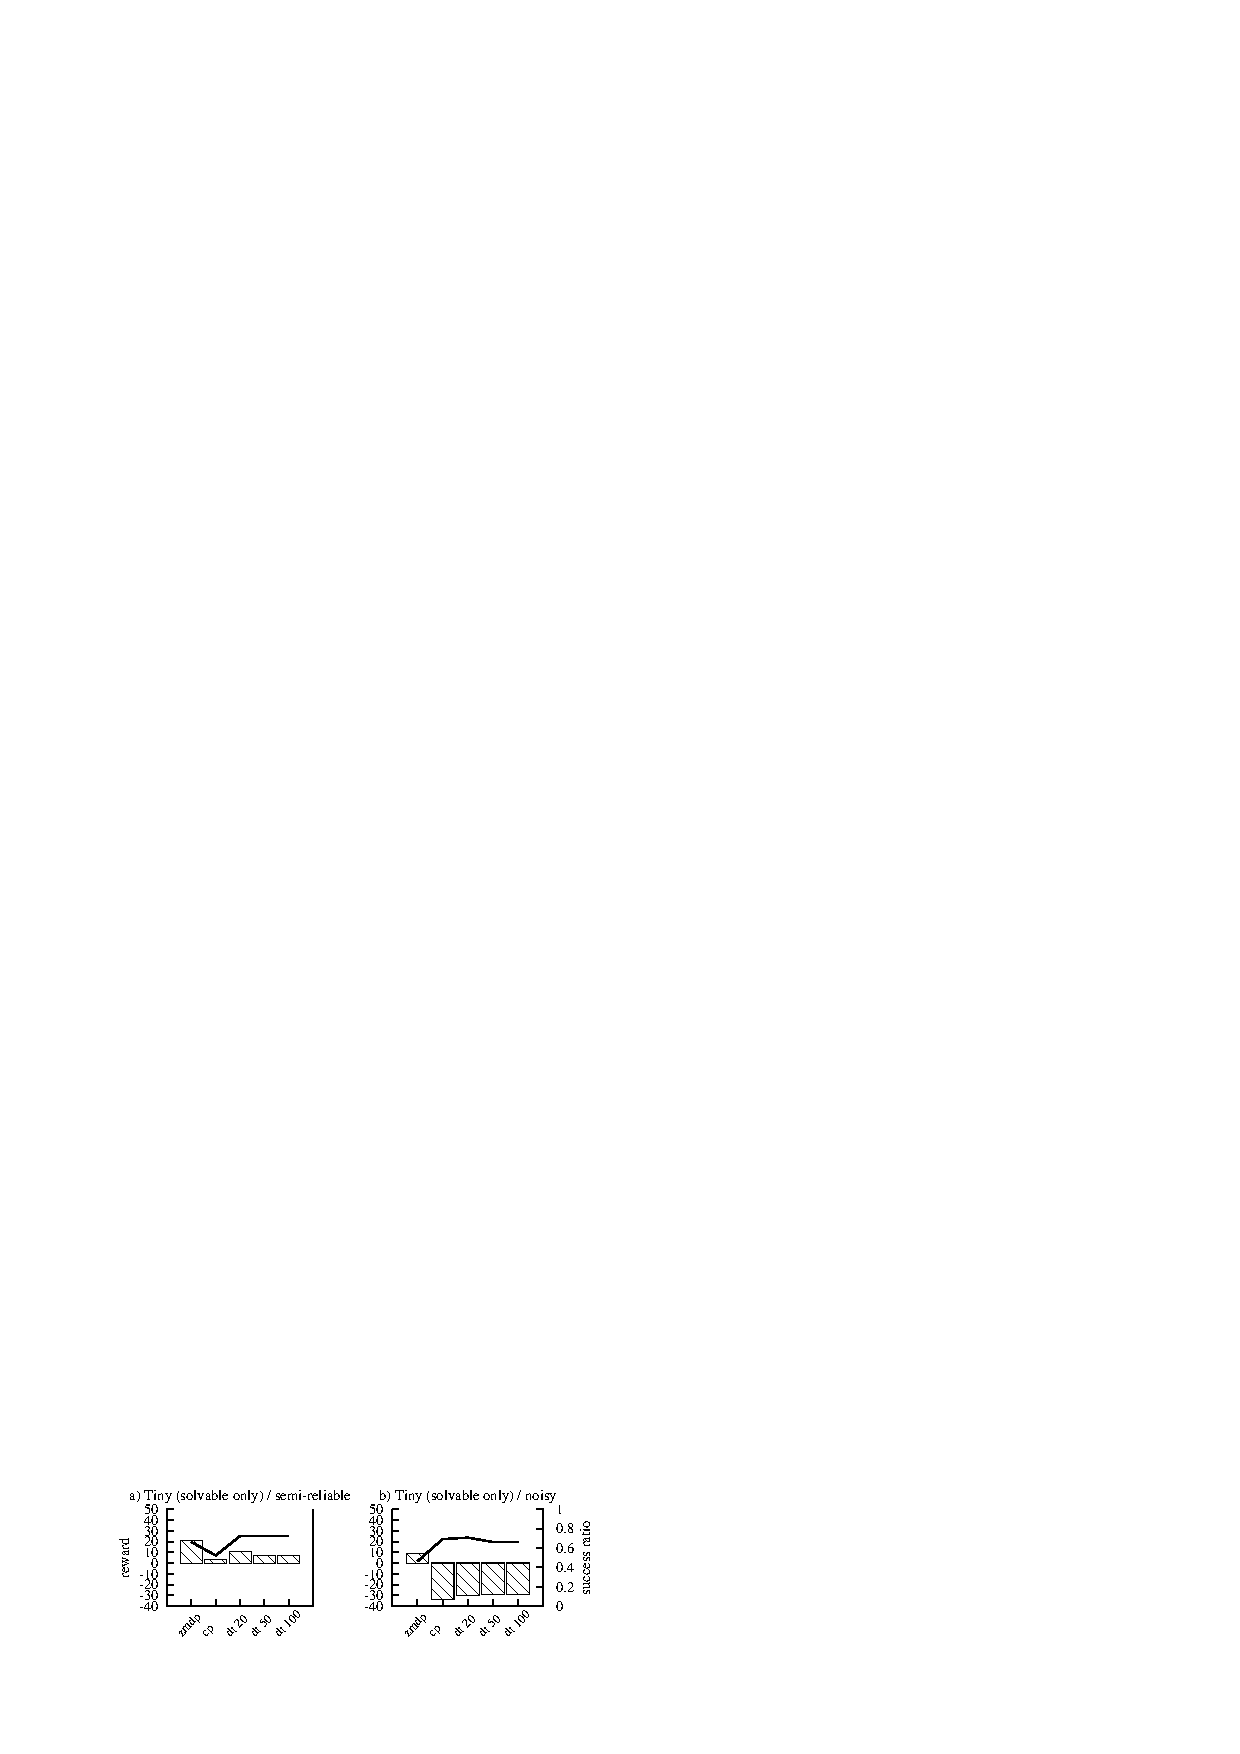
\includegraphics{pomdp-solvable-quality}\hfill
  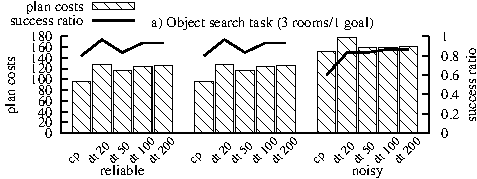
\includegraphics{dora2-quality}\hfill
  % \vspace{2mm}
  
\includegraphics{dora3-quality}\hfill
  % \vspace{2mm}
  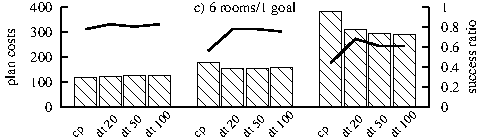
\includegraphics{dora4-quality}\hfill
  \vspace{2mm}
  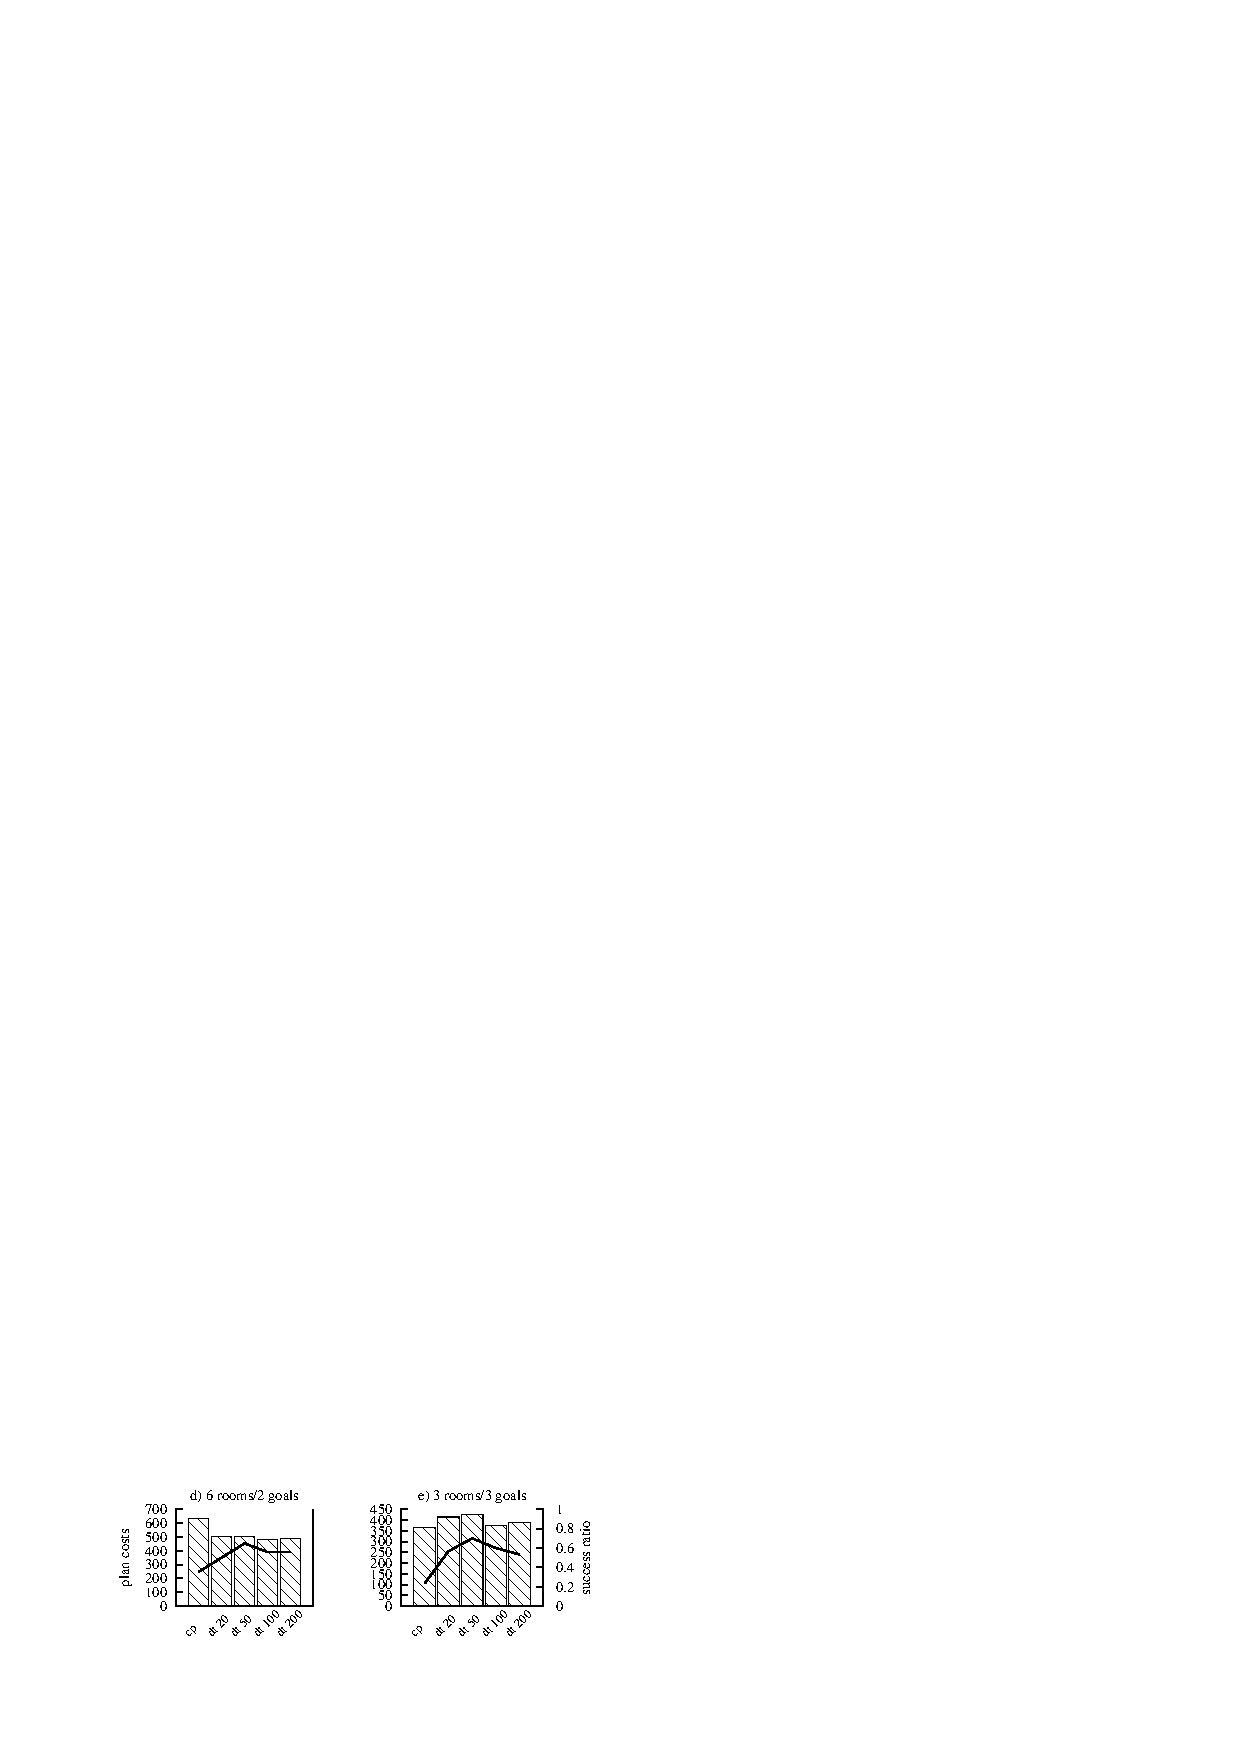
\includegraphics{dora56-quality}\hfill
  \vspace{2mm}
  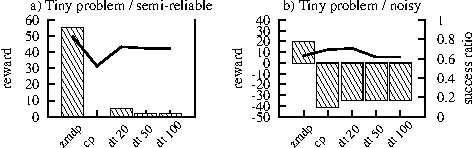
\includegraphics{pomdp-quality}\hfill
  % \vspace{2mm}
  % 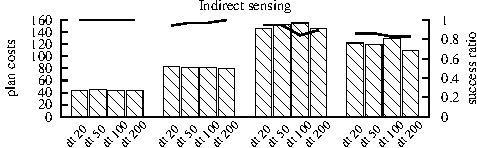
\includegraphics{dora-cat-quality}\hfill
  \caption{Average plan costs and number of successful runs.}
  \label{fig:results-quality}
\end{figure}

We find that if sensing is reliable there is little to be gained
through DT sessions, as the greedy approach of the {\em baseline} is
sufficient. As sensing degrades contingent planning pays off.  Time
spent in DT planning increases steeply as the abstraction $\bstate_0$
becomes more refined.  That refinement seems to be paying off in terms
of the success rate, particularly for tasks $d$ and $e$. For less
refined initial configurations, the increased cost of DT
planning is partially compensated for by a decrease in Fast Downward planning
times. The relatively high success rate irrespective of the level of
refinement in the initial configuration indicates the effectiveness of
using conditional entropy to guide abstraction refinement in our
setting.

%%% Local Variables: 
%%% mode: latex
%%% TeX-master: "aaai11"
%%% End: 


% We can put back in if desired
%
% \section{Limitations of Initial Approach}
% 
% The spatial transfer algorithm described in here has a number of limitations to be addressed in future work.  First, we have not incorporated a memory retrieval mechanism, such as MAC/FAC \cite{forbus/etal1995}.  As a cognitive system gains experience in different environments, it will have access to a range of context-dependent spatial regions defined in a variety of task situations. To retrieve an analogous example, the agent must select the most similar environment that contains a labeled example of the sought after region type. This extension is fairly straightforward, but beyond the scope of this paper. Second, our initial approach ignores a number of potentially relevant pieces of information. After the context-dependent spatial region has been identified in the target environment, its qualitative spatial relationships could be compared with those from the base to either refine the region or provide a confidence measure for the inference. In our example, the transferred region contains the bottom desk in the second row, but the corresponding region does not contain any desks topologically. Third, our algorithm uses an absolute reference frame. Therefore, the environments must be oriented in a similar fashion to successfully transfer a context-dependent spatial region. We can overcome this limitation by performing a series of analogies between the base and the target in which we rotate the base and select the analogy with the best mapping. Finally, more advanced qualitative spatial relationships should improve performance. For example, recognizing all the desks as one region, or grouping them into rows or columns, would provide a better level of abstraction for this task.

\section{Related Work}

% robots and space

Typical approaches to spatial representation for mobile robots tend to focus on localization, and thus mostly represent the world uniformly without subdivision into meaningful (semantic) units \cite{Thrun02a}. When a more structured representation is required, many turn to Kuipers' Spatial Semantic Hierarchy~\cite{Kuipers:2000}. This paper follows in this tradition, adding CDSRs to his qualitative topological representations. Whilst mobile robots exist which can determine the type of a room from the objects in it ~\cite{Hanheide/etal:2010a,Galindo/etal:2005a}, they only concern themselves with types of whole rooms, and cannot represent regions within rooms. This is also true for those systems which use some elements of QSR~\cite{aydemir2011icra}. The need for an autonomous system to ground references to human-generated descriptions of space has been recognized in domains where a robot must be instructed to perform a particular task, however existing systems are restricted to purely geometrically-defined regions~\cite{Tellex:2011,Dzifcak/etal:2009,brenneretal07ijcai}.


There is mounting evidence that analogy, operating over structured qualitative representations, can be used to simulate a number of spatial reasoning tasks. Forbus \textit{et al.} showed that analogy between course of action diagrams could be used to identify potential ambush locations in new situations by focusing on only the relevant aspects of sketched battle plans \cite{Forbus/etal2003}. A core contribution of their work was the definition of a \textit{shared similarity constraint} between a spatial reasoning system and its user; where users and spatial reasoning systems agree on the similarities between situations. This has close parallels to what we are trying to accomplish, where a cognitive system is able to reason about context-dependent spatial regions by identifying the same salient features as its human user. The anchor points in our work were originally used in teaching a system how to solve problems from the Bennett Mechanical Comprehension Test that require spatial and conceptual reasoning. For example, identifying which wheelbarrow will be more difficult to lift based on the relative locations of its loads as depicted in a sketch \cite{Klenk/etal2005}. In that work, the anchor points defined the endpoints of lines. We go beyond that result to use anchor points to specify 2D regions.  

% The combination of analogy and qualitative representation has been shown to be flexible enough to model problems at different levels of refinement (e.g. edges, shapes, groups) \cite{Lovett&Forbus2011} and to combine semantic as well as geometric information in spatial reasoning tasks (e.g. \cite{Lockwood/etal2008}). Our work demonstrates that the combination of analogy and qualitative spatial representations is useful for problems in cognitive mobile robotics. 
% Therefore, we hope and expect to see more research combining these three fields.

\section{Conclusion}

In this paper we presented an integrated cognitive system capable of representing and reasoning about context-dependent spatial regions. The system identifies CDSRs in previously unseen environments through analogy with a single example. This is a difficult cognitive systems task requiring integration of semantic and geometric knowledge to identify regions which can be as small as 8\% of the room. Our system demonstrates a successful integration of a range of technologies including vision, SLAM, qualitative spatial reasoning and analogy to achieve this task. In order to make this rich collection of components work together, our work takes a number of short-cuts that we plan to address with future work. These include a reliance on the initial orientation of a room in a global coordinate frame, the lack of a mechanism to retrieve relevant rooms from memory (e.g. MAC/FAC \cite{forbus/etal1995}), and a lack of transfer post-processing (e.g. comparing the QSRs present in both base and transferred regions) to improve results. In addition, we must complement our system development work with more comprehensive human studies assessing how people define and use these regions as well as how well anchor points capture them. Despite the preliminary nature of this work, our evaluation demonstrates that the system is able to produce CDSRs, which overlap with user-defined region, from a single example for 6 out of 7 region types.




% \section{Acknowledgments}
% 
% The authors would like to thank Jeffery Usher for providing the code to compute Voronoi diagrams, Scott Friedman for assistance on probablistic SME, and Danny Bobrow comments on an earlier draft of this paper. The research leading to these results has received funding from the European Community's Seventh Framework Programme [FP7/2007-2013] under grant agreement No. 215181, CogX.

% 7th page may only contain references
\clearpage

\bibliography{aaai12-cdsr}
\bibliographystyle{aaai}
\end{document}
